\begin{figure}[H]
    \center
    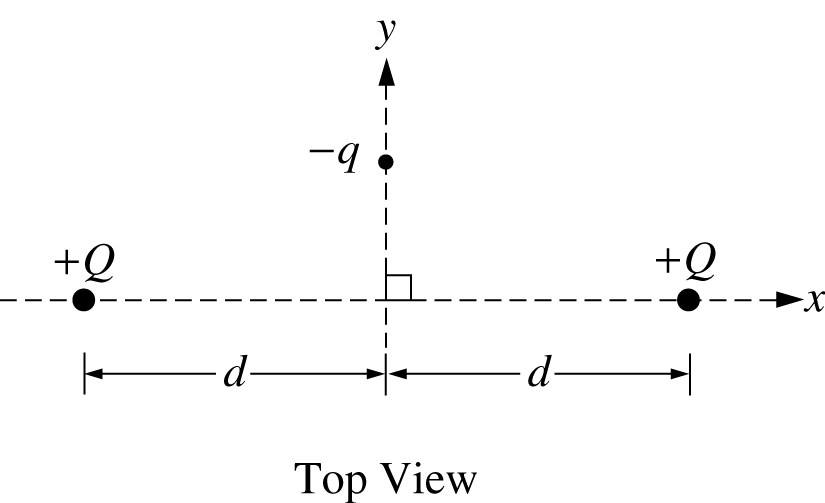
\includegraphics[scale=0.25]{images/img-007-016.png}
\end{figure}

% Multiple Choice Question 19
\begin{questions}\setcounter{question}{18}\question
Two objects on a horizontal frictionless surface each have charge $+Q$ and each are fixed in place on the $x$ axis at the same distance $d$ from the origin as shown in the figure above. A particle of charge $-q$ constrained to move along the $y$ axis is released from rest. After release, the particle will

\begin{choices}
\choice stay where it is
\choice exhibit oscillatory motion
\choice move in the direction of increasing $y$
\choice move in the direction of decreasing $y$ and stop at the origin
\choice move in the direction of decreasing $y$ and keep going to negative infinity
\end{choices}\end{questions}

